\documentclass[11pt,a4paper]{article}
\usepackage{gtu-el-yazisi}
\begin{document}
\notbilgi{Elektronik Elemanlar}{11. ve 12. Hafta -- MOSFET}{elektronik-elemanlar-11-ve-12.hafta.pdf}

\sayfa{1}
\section{11. hafta}

\begin{center}
\begin{circuitikz}
  \draw (0,0) node[nmos] (N) {};
  \draw (N.G) node[ocirc] {};
  \draw (N.D) node[above] {D};
  \draw (N.S) node[below] {S};
  \node at (0,-1.7) {Nmos};
  \draw (5,0) node[pmos] (P) {};
  \draw (P.G) node[ocirc] {};
  \draw (P.S) node[above] {S};
  \draw (P.D) node[below] {D};
  \node at (5.6,-1.7) {Pmos --- $V_{Tp}$ negatif};
\end{circuitikz}
\end{center}

\sekilnotu[1]{NMOS kesiti: p tipi gövde (içinde $+$ işaretleri, ``p''), yüzeyde iki $n$ bölgesi;
sol $n$ bölgesinden S, sağ $n$ bölgesinden D ucu, ortada oksit üzerinde G ucu, gövdenin altından
B ucu. Kapının altında, iki $n$ bölgesi arasında ``$-\,-\,-$'' ile gösterilen elektron kanalı;
ok ile ``inversion \okunamadi{condition}'' notu.}

\sekilnotu[1]{İkinci kesit (S, B, G, D uçları; iki $n$ bölgesi): kanal drain tarafında daralıp
$n$ bölgesine ulaşmadan kesiliyor; ok ile ``pinch off'' yazılmış.}

\begin{center}
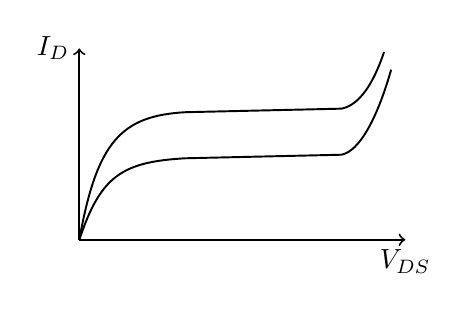
\begin{tikzpicture}[scale=0.9, line width=0.7pt]
  \draw[->] (0,0) -- (4.6,0) node[below] {$V_{DS}$};
  \draw[->] (0,0) -- (0,2.7) node[left] {$I_D$};
  \draw (0,0) .. controls (0.25,1.4) and (0.6,1.75) .. (1.5,1.8) -- (3.7,1.85)
        .. controls (3.95,1.9) and (4.15,2.2) .. (4.3,2.65);
  \draw (0,0) .. controls (0.3,0.9) and (0.6,1.1) .. (1.5,1.15) -- (3.7,1.2)
        .. controls (3.95,1.25) and (4.2,1.7) .. (4.4,2.4);
\end{tikzpicture}
\hspace{1.5cm}
\begin{tikzpicture}[scale=0.9, line width=0.7pt]
  \draw[->] (0,0) -- (3.8,0) node[right] {$V_{GS}$};
  \draw[->] (0,0) -- (0,2.7) node[left] {$I_D$};
  \draw (0,0) .. controls (1.4,0) and (1.9,0.5) .. (2.3,2.4);
\end{tikzpicture}
\end{center}

\noindent{\small\color{kursunkalem}(Sol kenarda yuvarlak içine alınmış iki kısa not: \okunamadi{}, \okunamadi{}.)}

\sayfa{2}
\subsection{Triode}
\[
  \boxed{I_D = k_n'\,\frac{W}{L}\left[\overbrace{(V_{GS}-V_{TH})}^{V_{ov}}V_{DS} - \frac{1}{2}V_{DS}^2\right]}
  \qquad\qquad \boxed{V_{DS} \le V_{GS}-V_{TH}}
\]
\[
  \phantom{I_D} = \frac{1}{2}\,k_n'\,\frac{W}{L}\left(2\,(V_{GS}-V_{TH})\,V_{DS} - V_{DS}^2\right)
\]

\subsection{Sat}
\[
  I_D = \frac{1}{2}\,k_n'\,\frac{W}{L}\,(V_{GS}-V_{TH})^2
  \qquad\qquad \boxed{V_{DS} \ge V_{GS}-V_{TH}}
\]

\subsection{Deep triode}
\[
  r = \frac{1}{\mu_n C_{ox}\,\frac{W}{L}\,(V_{GS}-V_{TH})}
\]

\noindent{\small\color{kursunkalem}(İki koşul kutusu çizgilerle aşağıdaki ``At the edge of saturation'' ifadesine bağlanmış.)}

\medskip
\noindent At the edge of saturation
\begin{align*}
  V_{DS} &= V_{GS} - V_{TH}\\
  V_D - V_S &= V_G - V_S - V_{TH}\\
  V_{TH} &= V_G - V_D\\
  V_{TH} &= V_{GD}
\end{align*}

\sekilnotu[2]{NMOS sembolü: G ucu sola ve yukarı uzatılmış, üst ucunda ``$+$''; D ucunun üstünde ``$-$'';
ikisi arasında $V_{Th}$ yazılı (yani $V_{GD}$). Yanında ``$\uparrow$ Triode'' ve ``$\downarrow$ Saturasyon'';
D ucunda aşağı yönlü akım oku ``$I=$''.}

\sayfa{3}
\noindent
\begin{minipage}[c]{0.3\linewidth}
\centering
\begin{circuitikz}
  \draw (0,0) node[nmos] (M) {};
  \draw (M.D) -- ++(0,0.5) coordinate (ust);
  \draw (M.G) |- (ust);
  \draw (ust) to[short,*-o] ++(0,0.4);
  \draw (M.S) to[short,-o] ++(0,-0.3);
\end{circuitikz}
\end{minipage}
\begin{minipage}[c]{0.6\linewidth}
Diode connected transistor
\end{minipage}

\begin{ornek}[2]
$0{,}18\,\mu$m process\\
$L = \qty{0,18}{\micro\metre}$, \ $W = \qty{2}{\micro\metre}$, \ $C_{ox} = 8{,}6\ \mathrm{fF}/\mu\mathrm{m}^2$,
\ $\mu_n = 450\ \mathrm{cm}^2/\mathrm{Vs}$, \ $V_{Tn} = 0{,}5\ \mathrm{V}$

a) $V_{GS} = ?$ \ $V_{DS} = ?$ \ at the edge of saturation. $I_D = 100\ \mu\mathrm{A}$
\end{ornek}
\begin{cozum}
\begin{align*}
  k_n' &= \mu_n C_{ox} = 450\cdot10^{-4}\cdot 8{,}6\cdot10^{-15}\cdot10^{12}\ \mathrm{A/V^2}\\
       &= 387\ \mu\mathrm{A/V^2}\\
  k_n &= k_n'\left(\frac{W}{L}\right) = 387\left(\frac{2}{0{,}18}\right) = 4{,}3\ \mathrm{mA/V^2}\\
  I_D &= \frac{1}{2}\,k_n\,(V_{ov})^2\\
  100 &= \frac{1}{2}(4{,}3)\cdot10^3\cdot(V_{ov})^2
\end{align*}
\[
  V_{ov} = 0{,}22\ \mathrm{V} \;\longrightarrow\; V_{DS} = V_{GS} - V_{TH} = 0{,}22
\]
\[
  \Big\downarrow\qquad V_{GS} = V_{TH} + V_{ov} = 0{,}5 + 0{,}22 = 0{,}72
\]
\end{cozum}

\noindent b) $V_{GS}$ is kept constant $\rightarrow$ $V_{DS} = ?$ when $I_D = 50\ \mu\mathrm{A}$
\hfill{\small(azaldı, grafiğe bak)}

\begin{cozum}
Triode bölgesi:
\begin{align*}
  I_D &= k_n\left[V_{ov}V_{DS} - \frac{1}{2}V_{DS}^2\right]\\
  50 &= 4{,}3\cdot10^3\left[0{,}22\,V_{DS} - \frac{1}{2}V_{DS}^2\right]
  \;\longrightarrow\; \boxed{V_{DS} = 0{,}06\ \mathrm{V}} \rightarrow \text{bunu alırız}
\end{align*}
\hfill $V_{DS} = $ \okunamadi{0,39} V $\rightarrow$ sat'ta
\[
  V_{DS} = 0{,}06\ \mathrm{V}
\]
\end{cozum}

\sayfa{4}
\noindent c) MOSFET $\rightarrow$ as a linear amplifier $\rightarrow$ (sat)\\[1mm]
\hspace*{1em}$\uparrow$\\
\hspace*{1em}$\{\,V_{DS} = 0{,}3\ \mathrm{V}$\\[1mm]
The change in $i_D$ resulting from
$V_{GS} \rightarrow 0{,}7\ \mathrm{V}
\begin{cases}
  \nearrow +0{,}01\ \mathrm{V} \Rightarrow i_D\,?\\
  \searrow -0{,}01\ \mathrm{V} \Rightarrow i_D\,?
\end{cases}$
\quad ($\leftarrow$ \underline{small signal})

\begin{cozum}
$V_{GS} = 0{,}7\ \mathrm{V}$, \ $V_{ov} = 0{,}2\ \mathrm{V}$ \hfill $(V_{TH} = 0{,}5\ \mathrm{V})$\\
$V_{DS} = 0{,}3\ \mathrm{V}$
\begin{align*}
  I_D &= \frac{1}{2}\,k_n\,(V_{ov})^2\\
      &= \frac{1}{2}\,4300\cdot 0{,}04\\
      &= 86\ \mu\mathrm{A}
\end{align*}

$V_{GS} = 0{,}71\ \mathrm{V} \Rightarrow V_{ov} = 0{,}21\ \mathrm{V}$\\
$V_{DS} = 0{,}3\ \mathrm{V} \Rightarrow \quad
  i_D = \frac{1}{2}\cdot 4300\,(0{,}21)^2 = 94{,}8\ \mu\mathrm{A}$

\medskip
$V_{GS} = 0{,}69\ \mathrm{V}$, \ $V_{ov} = 0{,}19\ \mathrm{V}$
\[
  i_D = \frac{1}{2}\cdot 4300\cdot(0{,}19)^2 = 77{,}6\ \mu\mathrm{A}
\]
\begin{align*}
  \Delta V_{GS} &= 0{,}01\ \mathrm{V} \;\rightarrow\; \Delta i_D = 8{,}8\ \mu\mathrm{A}\\
  \Delta V_{GS} &= -0{,}01\ \mathrm{V} \;\rightarrow\; \Delta i_D = -8{,}4\ \mu\mathrm{A}
\end{align*}
\end{cozum}

\sayfa{5}
\subsection{Örnek}
\sekilnotu[5]{PMOS sembolü: S üstte, G solda, D altta. S tarafında ``$+$'', G'de ``$-$'' ve aralarında
$|V_{THp}| + |V_{ov}|$ yazılı. Sağda S hizasından aşağı inen bir gerilim ölçeği: üstteki kısa aralık
``Triode'', sınır seviyesinden aşağı uzun aralık ``Sat.''; sınır seviyesinin hemen altında küçük bir
$|V_{THp}|$ oku. D ucundan çıkan çizgi sağa ve yukarı giderek bu sınır seviyesine bağlanıyor.}

\begin{ornek}[5.3]
\noindent
\begin{minipage}[c]{0.45\linewidth}
\centering
\begin{circuitikz}[scale=0.9, transform shape]
  \draw (0,0) node[nmos] (M) {};
  \draw (M.G) -- ++(-0.8,0) node[ground] {};
  \draw (M.D) to[R, l_=$R_D$, i<=$I_D$] ++(0,2) node[above] {$2{,}5$ V};
  \draw (M.D) to[short,-o] ++(1,0) node[right] {$V_D = 0{,}5$ V};
  \draw (M.S) to[R, l_=$R_S$, i>=$I_D$] ++(0,-2) node[below] {$-2{,}5$ V};
\end{circuitikz}
\end{minipage}\hfill
\begin{minipage}[c]{0.5\linewidth}
$I_D = 0{,}4\ \mathrm{mA}$, \ $V_{TH} = 0{,}7\ \mathrm{V}$, \ $\mu_n C_{ox} = 100\ \mu\mathrm{A/V^2}$\\
$L = 1\ \mu\mathrm{m}$, \ $W = 32\ \mu\mathrm{m}$\\
$(\lambda = 0)$
\end{minipage}
\end{ornek}
\begin{cozum}
$I_D = \frac{1}{2}\,\mu_n C_o$
\begin{align*}
  R_D &= \frac{V_{DD} - V_D}{I_D} = \frac{2{,}5 - 0{,}5}{0{,}4} = 5\ \mathrm{k\Omega}\\
  I_D &= \frac{1}{2}\,\mu_n C_{ox}\,\frac{W}{L}\,V_{ov}^2\\
  400 &= \frac{1}{2}\cdot 100\cdot\frac{32}{1}\,V_{ov}^2 \;\Rightarrow\; \boxed{V_{ov} = 0{,}5\ \mathrm{V}}
\end{align*}
\[
  \boxed{V_{GS} = 0{,}7 + 0{,}5 = 1{,}2\ \mathrm{V}}
\]
\[
  R_S = \frac{-1{,}2 - (-2{,}5)}{0{,}4} = 3{,}25\ \mathrm{k\Omega}
\]
\end{cozum}

\sayfa{6}
\subsection{ex: 5.4}
\noindent
\begin{minipage}[c]{0.3\linewidth}
\centering
\begin{circuitikz}
  \draw (0,0) node[nmos] (M) {};
  \draw (M.D) -- ++(0,0.5) coordinate (u);
  \draw (M.G) -- ++(-0.3,0) |- (u);
  \draw (u) to[short, *-o, i<=$i$] ++(0,0.7) node[right] {$+$};
  \draw (M.S) to[short, -o] ++(0,-0.4) node[right] {$-$};
  \node at (0.9,0) {$V$};
\end{circuitikz}
\end{minipage}
\begin{minipage}[c]{0.65\linewidth}
$\rightarrow$ Daima aynı bölgede
\[
  i = \frac{1}{2}\,k_n\,(V - V_{TH})^2
\]
\end{minipage}

\subsection{ex: 5.5}
\noindent
\begin{minipage}[c]{0.42\linewidth}
\centering
\begin{circuitikz}
  \draw (0,0) node[nmos] (M) {};
  \draw (M.G) -- ++(-0.3,0) -- ++(0,1.6) node[above] {$5$ V};
  \draw (M.D) to[R, l_=$R_D$] ++(0,1.8) node[above] {$5$ V};
  \draw (M.D) to[short, -o] ++(1.2,0) node[right] {$V_D = 0{,}1$ V};
  \draw (M.S) -- ++(0,-0.3) node[ground] {};
\end{circuitikz}\\[1mm]
\okunamadi{$V_{GD}>$} Deep triode
\end{minipage}\hfill
\begin{minipage}[c]{0.55\linewidth}
$V_{TH} = 1\ \mathrm{V}$, \ $k_n'\left(\frac{W}{L}\right) = 1\ \mathrm{mA/V^2}$\\[1mm]
$\rightarrow$ Effective resistance $\rightarrow \dfrac{V_{DS}}{I_{DS}} = ?$
\begin{align*}
  I_D &= k_n'\,\frac{W}{L}\left[(V_{GS}-V_{TH})\,V_{DS} - \frac{1}{2}V_{DS}^2\right]\\
  I_D &= 1\cdot\left[(5-1)(0{,}1) - \frac{1}{2}(0{,}1)^2\right]\\
      &= 0{,}395\ \mathrm{mA}
\end{align*}
\end{minipage}
\[
  R_{DS} = \frac{V_{DS}}{I_D} = \frac{0{,}1}{0{,}395} = 253\ \Omega
  \qquad\Big/\qquad
  R_{DS} = \frac{1}{k_n V_{ov}} \;\Rightarrow\; \frac{1}{1\cdot(5-1)} = 250\ \Omega
\]

\subsection{ex: 5.6}
\noindent
\begin{minipage}[c]{0.55\linewidth}
\centering
\begin{circuitikz}[scale=0.85, transform shape]
  \draw (0,0) node[nmos] (M) {};
  \draw (M.G) -- ++(-2.6,0) coordinate (g) node[midway, above] {$5$ V}
        node[midway, below] {$\overrightarrow{\ I=0\ }$};
  \draw (g) to[R, l=$R_{G1}$, a=$10\,\mathrm{M\Omega}$] ++(0,2.2) node[above] {$V_{DD} = 10$ V};
  \draw (g) to[R, l=$10\,\mathrm{M\Omega}$, a=$R_{G2}$, *-] ++(0,-2.2) node[ground] {};
  \draw (M.D) to[R, l_={$R_D = 6\,\mathrm{k\Omega}$}, i<=$I_D$] ++(0,2) node[above] {$10$ V};
  \draw (M.D) to[short, -*] ++(1,0) node[right] {D $\rightarrow V_D = 10 - 6I_D$};
  \draw (M.S) to[R, l_=$6\,\mathrm{k\Omega}$, i>=$I_D$] ++(0,-2) node[ground] {};
  \draw (M.S) to[short, -*] ++(1,0) node[right] {S $\rightarrow V_S = 6I_D$};
\end{circuitikz}
\end{minipage}\hfill
\begin{minipage}[c]{0.4\linewidth}
$V_{TH} = 1\ \mathrm{V}$, \ $k_n'(W/L) = 1\ \mathrm{mA/V^2}$, \ $(\lambda = 0)$\\
Determine all voltages and currents
\[
  V_G = V_{DD}\,\frac{R_{G2}}{R_{G2} + R_{G1}} = 10\,\frac{10}{10+10} = 5\ \mathrm{V}
\]
\end{minipage}

\medskip
\noindent
\begin{minipage}[t]{0.4\linewidth}
$\rightarrow$ Biasing\\
$I_D = 0{,}5\ \mathrm{mA}$\\
$V_S = 0{,}5\cdot 6 = 3\ \mathrm{V}$\\
$V_{GS} = 5 - 3 = 2\ \mathrm{V}$ \ ($\rightarrow\ > V_{TH}\ \checkmark$)\\
$V_D = 10 - 6\cdot 0{,}5 = 7\ \mathrm{V}$
\end{minipage}\hfill
\begin{minipage}[t]{0.56\linewidth}
$\leftarrow$ \ \underline{Varsayım 1: sat}
\begin{align*}
  I_D &= \frac{1}{2}\,k_n'\,\frac{W}{L}\,(V_{GS} - V_{TH})^2\\
  I_D &= \frac{1}{2}\cdot 1\cdot(5 - 6I_D - 1)^2\\
  18\,I_D^2 &- 25\,I_D + 8 = 0
\end{align*}
$I_D = 0{,}89$ (üstü çizili) \quad , \quad $\boxed{I_D = 0{,}5}$\\
{\small $\uparrow$ Bunu seçince $V_{GS}$ negatif olur}
\end{minipage}

\sayfa{7}
\section{12. hafta}
{\small\color{kursunkalem}Kenar notları: ``\okunamadi{BJT / Mosfet}'', ``Appendix \okunamadi{K}''}

\subsection{Comparison of the Mosfet and the BJT}
\noindent\underline{Typical values of CMOS device parameters}

\begin{center}
\resizebox{\linewidth}{!}{%
\begin{tabular}{l*{11}{c}}
\toprule
 & \multicolumn{2}{c}{$0{,}8\,\mu$m} & \multicolumn{2}{c}{$0{,}5\,\mu$m} & \multicolumn{2}{c}{$0{,}25\,\mu$m}
 & \multicolumn{2}{c}{$0{,}18\,\mu$m} & \multicolumn{2}{c}{$0{,}13\,\mu$m} & 65\,nm\\
\cmidrule(lr){2-3}\cmidrule(lr){4-5}\cmidrule(lr){6-7}\cmidrule(lr){8-9}\cmidrule(lr){10-11}\cmidrule(lr){12-12}
Parameter & NMOS & PMOS & NMOS & PMOS & NMOS & PMOS & NMOS & PMOS & NMOS & PMOS & NMOS\\
\midrule
$t_{ox}$     & 15  & 15     & 9   & 9      & 6   & 6      & 4    & 4      & 2,7  & 2,7    & 1,4\\
$C_{ox}$     & 2,3 & 2,3    & 3,8 & 3,8    & 5,8 & 5,8    & 8,6  & 8,6    & 12,8 & 12,8   & 25\\
$\mu$        & 550 & 250    & 500 & 180    & 460 & 160    & 450  & 100    & 400  & 100    & 216\\
$\mu C_{ox}$ & 127 & 58     & 190 & 68     & 267 & 93     & 387  & 86     & 511  & 128    & 540\\
$V_{TH0}$    & 0,7 & $-$0,7 & 0,7 & $-$0,8 & 0,5 & $-$0,6 & 0,5  & $-$0,5 & 0,4  & $-$0,4 & 0,35\\
$V_{DD}$     & 5   & 5      & 3,3 & 3,3    & 2,5 & 2,5    & 1,8  & 1,8    & 1,3  & 1,3    & 1,0\\
$|V_A'|$     & 25  & 20     & 20  & 10     & 5   & 6      & 5    & 6      & 5    & 6      & 3\\
$C_{ov}$     & 0,2 & 0,2    & 0,4 & 0,4    & 0,3 & 0,3    & 0,37 & 0,33   & 0,36 & 0,33   & 0,33\\
\bottomrule
\end{tabular}}
\end{center}
{\small(65\,nm sütununun PMOS kısmı sayfa kenarında kalmış, görünmüyor.)}

\noindent $\mu$ satırından ok: $\rightarrow$ NMOS'ta hep daha büyüktür çünkü taşıyıcı olarak \okunamadi{kul\ldots}

\medskip
\noindent Table 6.2 -- BJT
\begin{center}
\begin{tabular}{lcccc}
\toprule
 & \multicolumn{2}{c}{High voltage} & \multicolumn{2}{c}{Low voltage}\\
\cmidrule(lr){2-3}\cmidrule(lr){4-5}
Parameter & npn & lateral pnp & npn & lateral pnp\\
\midrule
$A_E$ ($\mu$m$^2$) & 500 & \okunamadi{900} & 2 & 2\\
$I_S$ (A) & $5\times10^{-15}$ & $2\cdot10^{-15}$ & $6\cdot10^{-18}$ & $6\cdot10^{-18}$\\
$\beta_0$ & 200 & 50 & 100 & 50\\
$V_A$ (V) & 130 & 50 & 35 & 30\\
$\tau_F$ & 0,35 ns & 30 ns & 10 ps & 650 ps\\
\bottomrule
\end{tabular}
\end{center}

\sayfa{8}
{\small\color{kursunkalem}Sol üst köşe: ``\okunamadi{Page 6.3}''}

\begin{ornek}[6.1]
a) NMOS $\rightarrow \dfrac{W}{L} = 10$, \ $0{,}18\,\mu$m process\\
\hspace*{1.5em}$V_{ov},\ V_{GS} = ?$ \ $\rightarrow I_D = 100\ \mu\mathrm{A}$, \ $(\lambda = 0)$\\
b) Table 6.2 $\rightarrow$ npn $\rightarrow$ low voltage process -- $I_C = 100\ \mu\mathrm{A}$
\end{ornek}
\begin{cozum}
\begin{align*}
  I_D &= \frac{1}{2}\,\mu_n C_{ox}\left(\frac{W}{L}\right)V_{ov}^2\\
  100\ \mu\mathrm{A} &= \frac{1}{2}\cdot 387\cdot 10\cdot V_{ov}^2 \;\Rightarrow\; 0{,}23\ \mathrm{V} = V_{ov}\\
  V_{GS} &= V_{TH} + V_{ov} = 0{,}5 + 0{,}23 = 0{,}73\ \mathrm{V}
\end{align*}
b) $I_C = 100\ \mu\mathrm{A}$ \qquad $I_C = I_S\,e^{V_{BE}/V_T} \;\rightarrow\; I_S = 6\cdot10^{-18}$
\[
  \hookrightarrow\; V_{BE} = 0{,}025\,\ln\frac{100\cdot10^{-6}}{6\cdot10^{-18}} = 0{,}76\ \mathrm{V}
\]
\end{cozum}

\subsection{Table 6.3}
\sekilnotu[8]{NMOS sembolü (üstünde ``NMOS''): D ucuna giren $I_D$; G--D arasında $V_{GD}$ (G'de $+$, D'de $-$),
D--S arasında $V_{DS}$ (D'de $+$, S'de $-$), G--S arasında $V_{GS}$ (G'de $+$, S'de $-$).}

\noindent
\begin{tabular}{@{}p{0.14\linewidth}p{0.8\linewidth}@{}}
Active reg. &
\textcircled{\small 1}\quad $V_{GS} \ge V_{TH}$, \ $V_{TH} \approx 0{,}3\ \mathrm{V} - 0{,}5\ \mathrm{V}$\newline
\hspace*{1.6em}$V_{GS} = V_{TH} + V_{ov}$
\end{tabular}

\noindent\rule{0.6\linewidth}{0.4pt}

\noindent\hspace*{0.14\linewidth}\textcircled{\small 2}\quad Pinch off
\begin{align*}
  & V_{GD} < V_{TH}\\
  & V_{DS} > V_{ov}, \quad V_{ov} \approx 0{,}1\ \mathrm{V} \longleftrightarrow 0{,}3\ \mathrm{V}\\
  & I_D = \frac{1}{2}\,\mu_n C_{ox}\,\frac{W}{L}\,(V_{GS} - V_{TH})^2\left(1 + \frac{V_{DS}}{V_A}\right)\\
  & I_G = 0
\end{align*}

\noindent\rule{\linewidth}{0.4pt}

\sekilnotu[8]{npn BJT sembolü: C ucuna giren $I_C$, E ucundan çıkan $I_E$; B--C arasında $V_{BC}$
(B'de $+$, C'de $-$), B--E arasında $V_{BE}$ (B'de $+$, E'de $-$).}

\noindent $V_{BE} \ge V_{BE\,on}$, \quad $V_{BE\,on} \approx 0{,}5$, \quad Forward bias (EBJ)\\
Reverse bias\\
\hspace*{1.5em}$V_{BC} < V_{BC\,on}$, \quad $V_{BC\,on} \approx 0{,}4\ \mathrm{V}$\\
\hspace*{3em}$V_{CE} \ge 0{,}3\ \mathrm{V}$
\[
  I_C = I_S\,e^{V_{BE}/V_T}\left(1 + \frac{V_{CE}}{V_A}\right)
\]
\[
  I_B = \frac{I_C}{\beta}
\]

\sayfa{9}
{\small\color{kursunkalem}Üstte silik kurşun kalem notu: \okunamadi{Learn chapter \ldots\ circuits}}

\subsection{Small signal}
\noindent
\begin{minipage}[t]{0.52\linewidth}
\centering
\underline{NMOS}\\[1mm]
\begin{circuitikz}[scale=0.85, transform shape]
  \draw (0,2) node[ocirc] {} -- (1,2);
  \node at (0.6,1.7) {$+$};
  \node at (0.6,1.15) {$v_{gs}$};
  \node at (0.6,0.45) {$-$};
  \draw (0.4,0) -- (4.8,0);
  \draw (2.5,2) to[cI, l=$g_m v_{gs}$] (2.5,0);
  \draw (2.5,2) -- (4.8,2) to[short, -o] (5.6,2);
  \draw (4.8,2) to[R, l=$r_o$] (4.8,0);
\end{circuitikz}\\
$r_o \rightarrow \left(\dfrac{1}{\lambda I_D}\right)$
\begin{align*}
  \text{\small geçiş iletkenliği } g_m &= \frac{I_D}{V_{ov}/2}\\[-1mm]
  \text{\small (Transconductance)}\quad &\\
  g_m &= \mu_n C_{ox}\,\frac{W}{L}\,V_{ov}\\
  g_m &= \sqrt{2\,\mu_n C_{ox}\,\frac{W}{L}\,I_D}
\end{align*}
\end{minipage}\hfill\vrule\hfill
\begin{minipage}[t]{0.42\linewidth}
\centering
\underline{npn}\\[1mm]
\begin{circuitikz}[scale=0.85, transform shape]
  \draw (0,2) node[ocirc] {} -- (1.2,2) to[R, l=$r_\pi$] (1.2,0);
  \node at (0.5,1.5) {$+$};
  \node at (0.5,1.0) {$v_\pi$};
  \node at (0.5,0.45) {$-$};
  \draw (1.2,0) -- (5.6,0);
  \draw (2.6,0) to[short, -o] (2.6,-0.5) node[below] {E};
  \draw (3.2,2) to[cI, l=$g_m v_\pi$] (3.2,0);
  \draw (3.2,2) -- (5.6,2) to[short, -o] (6.4,2);
  \draw (5.6,2) to[R, l=$r_o$] (5.6,0);
\end{circuitikz}
\begin{align*}
  g_m &= I_C/V_T\\
  r_o &= V_A/I_C\\
  r_\pi &= \beta/g_m
\end{align*}
\end{minipage}

\begin{ornek}[6.2]
$0{,}25\,\mu$m process $\rightarrow g_m,\ r_o,\ A_o \rightarrow$ intrinsic gain $\rightarrow A_o = g_m\cdot r_o$, \ $R_{in}$?\\
npn $\rightarrow 100\ \mu\mathrm{A}$, \ $L = 0{,}4\ \mu\mathrm{m}$, \ $W = 4\ \mu\mathrm{m}$

\begin{center}
\begin{circuitikz}[scale=0.7, transform shape]
  \draw (0,0) node[nmos] {};
  \node at (-1.3,-0.5) {(CMOS)};
  \draw (2.5,0) node[npn] {};
\end{circuitikz}
\end{center}
\end{ornek}
\begin{cozum}
\begin{align*}
  I_D &= \frac{1}{2}\,\mu_n C_{ox}\,\frac{W}{L}\,V_{ov}^2 \;\rightarrow\\
  100 &= \frac{1}{2}\cdot 267\cdot\frac{4}{0{,}4}\cdot V_{ov}^2
\end{align*}
MOSFET $\rightarrow V_{ov} = 0{,}27\ \mathrm{V}$
\begin{align*}
  g_m &= \sqrt{2\,(\mu_n C_{ox})\left(\frac{W}{L}\right)I_D} = 0{,}73\ \mathrm{mA/V}\\
  R_{in} &= \infty, \qquad r_o = \frac{V_A' L}{I_D} = 20\ \mathrm{k\Omega}\\
  A_o &= g_m r_o = (0{,}73)(20) = 14{,}6\ \mathrm{V/V}
\end{align*}
\noindent\rule{0.6\linewidth}{0.4pt}
\begin{align*}
  g_m &= \frac{I_C}{V_T} = \frac{0{,}1}{0{,}025} = 4\ \mathrm{mA/V}\\
  R_{in} &= r_\pi = \frac{\beta}{g_m} = \frac{100}{40}\text{\textsuperscript{*}} = 25\ \mathrm{k\Omega}\\
  r_o &= \frac{V_A}{I_C} = \frac{35}{0{,}1} = 350\ \mathrm{k\Omega}\\
  A_o &= g_m r_o = 4\cdot 350 = 1400\ \mathrm{V/V}
\end{align*}
{\footnotesize\color{kursunkalem}* Claude notu: muhtemelen $\frac{100}{4}$ olmalı ($g_m = 4\ \mathrm{mA/V}$ ile $r_\pi = 25\ \mathrm{k\Omega}$).\par}
\end{cozum}

\sayfa{10}
{\small\color{kursunkalem}Sol üst köşede silik not: \okunamadi{}}

\subsection{JFET $\rightarrow$ Junction field effect transistor}

\sekilnotu[10]{JFET kesiti: ortada $n$ kanal (üstte ``Channel''), sağında ve solunda birer $p$ bölgesi;
iki $p$ bölgesi birbirine bağlı ve G ucuna (``(G)'') çıkıyor; D ucu üstte, S ucu altta.}

\begin{center}
\begin{circuitikz}
  \draw (0,0) node[njfet] (N) {};
  \draw (N.G) node[ocirc] {} node[left] {G};
  \draw (N.D) node[ocirc] {} node[above] {D};
  \draw (N.S) node[ocirc] {} node[below] {S};
  \node at (0,-1.4) {n-JFET};
  \draw (3,0) node[pjfet] (P) {};
  \draw (P.G) node[ocirc] {} node[left] {G};
  \draw (P.S) node[ocirc] {} node[above] {S};
  \draw (P.D) node[ocirc] {} node[below] {D};
  \node at (3,-1.4) {p-JFET};
\end{circuitikz}
\end{center}

\sekilnotu[10]{JFET (kutu olarak çizilmiş; G solda, D üstte, S altta) ile devre: G--S arasında ayarlı
bir gerilim kaynağı ($i_G = 0$), D--S arasında ``$V_{DS}$ small'' kaynağı ($+$ üstte).}

\noindent $V_P \rightarrow$ pinch off\\
Cut off \ $V_{GS} \le V_P$, \ $i_D = 0$

\sekilnotu[10]{JFET kesiti: iki $p$ bölgesi ve aralarındaki kanal; kesikli çizgilerle drain (üst) tarafına
doğru genişleyen fakirleşme bölgeleri. $p$ bölgesi ile alt (S) uç arasında $V_{GS}$ kaynağı, üst (D) uç ile
alt uç arasında ayarlı $V_{DS}$ kaynağı ($+$ üstte).}

\noindent Saturation (pinch off) \quad $V_P \le V_{GS} < 0$
\begin{gather*}
  V_{DS} \ge V_{GS} - V_P\\
  i_D = I_{DSS}\left(1 - \frac{V_{GS}}{V_P}\right)^2(1 + \lambda V_{DS})
\end{gather*}
Triode \quad $V_P \le V_{GS} \le 0$, \quad $V_{DS} \le V_{GS} - V_P$
\[
  i_D = I_{DSS}\left[2\left(1 - \frac{V_{GS}}{V_P}\right)\left(\frac{V_{DS}}{-V_P}\right) - \left(\frac{V_{DS}}{V_P}\right)^2\right]
\]

\begin{ornek}[(PS 4.7)]
\noindent
\begin{minipage}[c]{0.42\linewidth}
\centering
\begin{circuitikz}[scale=0.85, transform shape]
  \draw (0,0) node[njfet] (J) {};
  \draw (J.G) -- ++(-1.6,0) coordinate (g);
  \draw (g) to[R, l=$R_{G1}$, *-] ++(0,2.2);
  \draw (g) to[R, l_=$R_{G2}$] ++(0,-2.2) node[ground] {};
  \draw (J.D) to[R, l_=$R_D$] ++(0,2);
  \draw (J.D) to[short, -o] ++(0.9,0) node[right] {$11$ V};
  \draw (J.S) to[R, l=$R_S$] ++(0,-1.8) node[ground] {};
\end{circuitikz}
\end{minipage}\hfill
\begin{minipage}[c]{0.55\linewidth}
$V_P = -3\ \mathrm{V}$, \ $I_{DSS} = 9\ \mathrm{mA}$, \ $\lambda = 0$\\
$V_G = 5\ \mathrm{V}$, \ $I_D = 4\ \mathrm{mA}$, \ $V_D = 11\ \mathrm{V}$\\
Design for $0{,}05\ \mathrm{mA}$
\end{minipage}
\end{ornek}
\begin{cozum}
\[
  15\cdot\frac{R_{G2}}{R_{G1} + R_{G2}} = 5\ \mathrm{V} \;\Rightarrow\;
  \begin{array}{l} R_{G1} = x\\ R_{G2} = 2x \end{array}\text{\textsuperscript{*}}
\]
{\footnotesize\color{kursunkalem}* Claude notu: muhtemelen $R_{G1} = 2x$, $R_{G2} = x$ olmalı (aşağıdaki sonuç değerleriyle uyumlu).\par}
\[
  \frac{15}{3x} = 0{,}05\ \mathrm{mA} \;\Longrightarrow\; x = 100\ \mathrm{k\Omega}
  \qquad
  \begin{array}{l} R_{G1} = 200\ \mathrm{k\Omega}\\ R_{G2} = 100\ \mathrm{k\Omega} \end{array}
\]
\[
  R_D = \frac{15 - 11}{4\ \mathrm{mA}} = 1\ \mathrm{k\Omega}
\]
\[
  V_{DS} \ge V_{GS} - V_P \;\Rightarrow\; V_D > V_G + 3
\]
\hspace*{0.45\linewidth}$\downarrow$\\
\hspace*{0.42\linewidth}$11 > 5 + 3 \;\rightarrow\; 11 > 8$\\
\hspace*{0.3\linewidth}$\rightarrow$ (pinch-off)
\end{cozum}

\sayfa{11}
\begin{cozum}
\begin{gather*}
  I_D = I_{DSS}\left(1 - \frac{V_{GS}}{V_P}\right)^2\\
  \sqrt{\frac{4}{9}} = \left(1 - \frac{V_{GS}}{V_P}\right) \;\Rightarrow\; \frac{2}{3} = 1 + \frac{V_{GS}}{3}\\
  V_{GS} = 1\text{\textsuperscript{*}}
\end{gather*}
{\footnotesize\color{kursunkalem}* Claude notu: muhtemelen $V_{GS} = -1$ V olmalı ($V_S = 5 - (-1) = 6$ V ile uyumlu).\par}
$V_S = 6\ \mathrm{V}$
\[
  R_S = \frac{6}{4\mathrm{m}} = 1{,}5\ \mathrm{k\Omega}
\]
\[
  i_G = 0 \quad \text{her zaman}
\]
\end{cozum}

\noindent\rule{\linewidth}{0.4pt}

\begin{center}
ELM 231 Proje: Son teslim 28.11.2022
\end{center}

\noindent
\begin{circuitikz}[scale=0.8, transform shape]
  \draw (0,3) to[R, l_=$R_1$] (0,1.5) to[R, l_=$R_2$] (0,0);
  \draw (0,1.5) -- (1.8,1.5);
  \draw (1.8,1.2) -- (1.8,1.9);
\end{circuitikz}

\end{document}
